\documentclass{article} % For LaTeX2e
\usepackage{iclr2024_conference,times}

\usepackage[utf8]{inputenc} % allow utf-8 input
\usepackage[T1]{fontenc}    % use 8-bit T1 fonts
\usepackage{hyperref}       % hyperlinks
\usepackage{url}            % simple URL typesetting
\usepackage{booktabs}       % professional-quality tables
\usepackage{amsfonts}       % blackboard math symbols
\usepackage{nicefrac}       % compact symbols for 1/2, etc.
\usepackage{microtype}      % microtypography
\usepackage{titletoc}

\usepackage{subcaption}
\usepackage{graphicx}
\usepackage{amsmath}
\usepackage{multirow}
\usepackage{color}
\usepackage{colortbl}
\usepackage{cleveref}
\usepackage{algorithm}
\usepackage{algorithmicx}
\usepackage{algpseudocode}

\DeclareMathOperator*{\argmin}{arg\,min}
\DeclareMathOperator*{\argmax}{arg\,max}

\graphicspath{{../}} % To reference your generated figures, see below.
\begin{filecontents}{references.bib}

@book{goodfellow2016deep,
  title={Deep learning},
  author={Goodfellow, Ian and Bengio, Yoshua and Courville, Aaron and Bengio, Yoshua},
  volume={1},
  year={2016},
  publisher={MIT Press}
}

@article{vaswani2017attention,
  title={Attention is all you need},
  author={Vaswani, Ashish and Shazeer, Noam and Parmar, Niki and Uszkoreit, Jakob and Jones, Llion and Gomez, Aidan N and Kaiser, {\L}ukasz and Polosukhin, Illia},
  journal={Advances in neural information processing systems},
  volume={30},
  year={2017}
}

@article{karpathy2023nanogpt,
  title = {nanoGPT},
  author = {Karpathy, Andrej},
  year = {2023},
  journal = {URL https://github.com/karpathy/nanoGPT/tree/master},
  note = {GitHub repository}
}

@article{kingma2014adam,
  title={Adam: A method for stochastic optimization},
  author={Kingma, Diederik P and Ba, Jimmy},
  journal={arXiv preprint arXiv:1412.6980},
  year={2014}
}

@article{ba2016layer,
  title={Layer normalization},
  author={Ba, Jimmy Lei and Kiros, Jamie Ryan and Hinton, Geoffrey E},
  journal={arXiv preprint arXiv:1607.06450},
  year={2016}
}

@article{loshchilov2017adamw,
  title={Decoupled weight decay regularization},
  author={Loshchilov, Ilya and Hutter, Frank},
  journal={arXiv preprint arXiv:1711.05101},
  year={2017}
}

@article{radford2019language,
  title={Language Models are Unsupervised Multitask Learners},
  author={Radford, Alec and Wu, Jeff and Child, Rewon and Luan, David and Amodei, Dario and Sutskever, Ilya},
  year={2019}
}

@article{bahdanau2014neural,
  title={Neural machine translation by jointly learning to align and translate},
  author={Bahdanau, Dzmitry and Cho, Kyunghyun and Bengio, Yoshua},
  journal={arXiv preprint arXiv:1409.0473},
  year={2014}
}

@article{paszke2019pytorch,
  title={Pytorch: An imperative style, high-performance deep learning library},
  author={Paszke, Adam and Gross, Sam and Massa, Francisco and Lerer, Adam and Bradbury, James and Chanan, Gregory and Killeen, Trevor and Lin, Zeming and Gimelshein, Natalia and Antiga, Luca and others},
  journal={Advances in neural information processing systems},
  volume={32},
  year={2019}
}

@misc{gpt4,
  title={GPT-4 Technical Report}, 
  author={OpenAI},
  year={2024},
  eprint={2303.08774},
  archivePrefix={arXiv},
  primaryClass={cs.CL},
  url={https://arxiv.org/abs/2303.08774}, 
}
\end{filecontents}

\title{FactorSAE: Memory-Efficient Knowledge Editing via Low-Rank Matrix Decomposition}

\author{LLM\\
Department of Computer Science\\
University of LLMs\\
}

\newcommand{\fix}{\marginpar{FIX}}
\newcommand{\new}{\marginpar{NEW}}

\begin{document}

\maketitle

\begin{abstract}
Selective knowledge modification in large language models is crucial for model maintenance and updating, yet current approaches struggle with memory efficiency and precise targeting of specific information. We present FactorSAE, a memory-efficient sparse autoencoder architecture that enables knowledge editing through low-rank matrix factorization and block-diagonal feature isolation. Our method decomposes the weight matrices of Gemma-2B into low-rank components $(U, V) \in \mathbb{R}^{2304 \times 128}$, achieving 90\% memory reduction while maintaining model functionality. The architecture employs a block-diagonal structure with 32 feature clusters, combining streaming SVD updates and alternating optimization with orthogonality constraints for stable training. We evaluate our approach on five specialized datasets including WMDP-bio and computer science knowledge, demonstrating stable convergence through loss curves and feature sparsity analysis. While achieving significant memory efficiency and stable training dynamics, current experiments yield unlearning scores of 0.0 across all configurations, highlighting specific challenges in selective knowledge removal. Our work establishes a foundation for memory-efficient model maintenance while identifying key directions for improving precise knowledge modification in large language models.
\end{abstract}

\section{Introduction}
\label{sec:intro}

Large language models (LLMs) have demonstrated remarkable capabilities across diverse tasks \cite{gpt4}, but maintaining and updating their knowledge remains a significant challenge. As these models are deployed in real-world applications, the ability to selectively modify their learned information becomes crucial for correcting errors, removing harmful content, and keeping knowledge current \cite{goodfellow2016deep}. However, existing approaches to knowledge editing often require extensive computational resources and struggle to precisely target specific information without affecting other model capabilities.

The key challenge lies in the distributed nature of neural networks' knowledge representation. Unlike traditional databases with discrete entries, information in LLMs is encoded across millions of interconnected parameters \cite{vaswani2017attention}. This distributed structure creates three fundamental difficulties: (1) isolating specific knowledge components without disrupting others, (2) maintaining memory efficiency during modification, and (3) ensuring stable training dynamics throughout the editing process.

We address these challenges through FactorSAE, a novel sparse autoencoder architecture that enables memory-efficient knowledge editing through low-rank matrix factorization. Our approach decomposes the weight matrices $(W_{\text{enc}}, W_{\text{dec}}) \in \mathbb{R}^{2304 \times 2304}$ of Gemma-2B into low-rank components $W = UV^T$, where $U, V \in \mathbb{R}^{2304 \times 128}$. This factorization reduces memory requirements by 90\% while preserving model functionality through a block-diagonal structure with 32 feature clusters.

The key technical innovations of our work include:
\begin{itemize}
    \item A memory-efficient architecture that combines low-rank factorization with block-diagonal constraints, reducing parameters by 90\% while maintaining reconstruction quality
    \item A streaming optimization strategy that alternates between $U$ and $V$ matrices with periodic orthogonality enforcement every 100 steps, ensuring stable training
    \item A gradient-guided feature attribution mechanism that tracks importance over a 100-batch history window, enabling targeted knowledge modification
\end{itemize}

We evaluate our approach on five specialized datasets (WMDP-bio, high school US history, college computer science, high school geography, and human aging) using the Gemma-2B model. Our experiments demonstrate:
\begin{itemize}
    \item Successful implementation of memory-efficient transformations with stable convergence (Figure~\ref{fig:first_figure}b)
    \item Effective feature sparsification through L1 regularization ($\lambda_1 = 0.04$) and orthogonality constraints ($\lambda_2 = 0.1$)
    \item Current limitations in selective knowledge removal, with unlearning scores of 0.0 across all configurations
\end{itemize}

While our method achieves significant efficiency gains and stable training dynamics, the unlearning results highlight specific challenges in precise knowledge modification. These findings motivate future work in three directions: (1) dynamic rank adaptation to better balance compression and editability, (2) enhanced feature attribution mechanisms for improved knowledge isolation, and (3) alternative block-diagonal structures that better align with natural knowledge boundaries in the model \cite{radford2019language}.

\section{Related Work}
\label{sec:related}

Our approach to memory-efficient knowledge editing builds upon three key research directions, each offering distinct insights and limitations for our problem setting.

\subsection{Knowledge Editing in Language Models}
While attention mechanisms \cite{vaswani2017attention} enable flexible information routing, they complicate targeted knowledge modification due to distributed representations. Unlike our block-diagonal approach, standard fine-tuning methods \cite{radford2019language} modify all parameters indiscriminately, risking catastrophic forgetting. In contrast, our method isolates knowledge components through sparse feature clusters, though achieving 0.0 unlearning scores indicates this remains challenging.

\subsection{Low-Rank Model Compression}
Traditional compression techniques like pruning and quantization \cite{goodfellow2016deep} focus on reducing model size without considering knowledge editability. Our work differs by using matrix factorization specifically for knowledge isolation, decomposing $2304 \times 2304$ matrices into $2304 \times 128$ components. While this achieves 90\% memory reduction similar to standard compression, our block-diagonal structure with 32 feature clusters enables more targeted modifications than general compression methods.

\subsection{Sparse Representations for Model Adaptation}
Layer-specific adaptation approaches \cite{ba2016layer} and optimization techniques \cite{kingma2014adam} typically add new parameters rather than modifying existing knowledge. Our sparse autoencoder architecture instead explicitly decomposes knowledge into interpretable features through alternating optimization and orthogonality constraints. This enables more precise targeting than full fine-tuning, though our current 0.0 unlearning scores suggest the need for improved feature isolation mechanisms.

\section{Background}
\label{sec:background}

Our work builds upon three foundational areas: transformer architectures, sparse autoencoders, and low-rank matrix approximations. The transformer architecture \cite{vaswani2017attention} enables flexible information routing through attention mechanisms, but its distributed knowledge representation poses challenges for selective modification. Each layer processes information through key-query-value transformations with dense weight matrices $W \in \mathbb{R}^{d \times d}$, where $d=2304$ in our target Gemma-2B model.

Sparse autoencoders \cite{goodfellow2016deep} provide a framework for decomposing these dense representations into interpretable features. An autoencoder consists of an encoder $E: \mathbb{R}^d \rightarrow \mathbb{R}^n$ and decoder $D: \mathbb{R}^n \rightarrow \mathbb{R}^d$, where sparsity constraints encourage disentangled representations. This sparsity is typically enforced through L1 regularization, though maintaining stability requires careful optimization \cite{kingma2014adam}.

Low-rank matrix factorization offers memory-efficient approximations while preserving essential structure. For a weight matrix $W$, we seek factors $U, V$ such that $W \approx UV^T$ minimizes the Frobenius norm $\|W - UV^T\|_F$ subject to rank constraints. The factorization's effectiveness depends on the true rank of $W$ and the chosen approximation rank.

\subsection{Problem Setting}
\label{subsec:problem}

Let $\mathcal{M}$ be a pre-trained language model with parameters $\theta$ and hidden dimension $d$. Given a subset of knowledge $\mathcal{K}$ to be modified, we seek a memory-efficient transformation $\mathcal{T}: \mathbb{R}^d \rightarrow \mathbb{R}^d$ that can:
\begin{enumerate}
    \item Isolate $\mathcal{K}$ through sparse feature activations
    \item Modify $\mathcal{K}$ while preserving other capabilities
    \item Maintain reconstruction quality with reduced parameters
\end{enumerate}

Formally, we structure $\mathcal{T}$ as a factorized autoencoder:
\begin{equation}
    \mathcal{T}(x) = D(E(x)) = (U_{\text{dec}}V_{\text{dec}}^T)(U_{\text{enc}}V_{\text{enc}}^T x + b_{\text{enc}}) + b_{\text{dec}}
\end{equation}
where $U_{\text{enc}}, V_{\text{enc}}, U_{\text{dec}}, V_{\text{dec}} \in \mathbb{R}^{d \times r}$ with $r \ll d$ and $b_{\text{enc}}, b_{\text{dec}} \in \mathbb{R}^d$.

Our approach makes three key assumptions:
\begin{itemize}
    \item The knowledge in $\mathcal{K}$ can be isolated through sparse feature activations
    \item A rank-$r$ approximation ($r=128$) preserves sufficient information
    \item Knowledge exhibits natural clustering that aligns with block-diagonal structure
\end{itemize}

These assumptions are motivated by empirical observations in transformer models \cite{vaswani2017attention} and validated through our experimental results in Section \ref{sec:results}.

\section{Method}
\label{sec:method}

Building on the problem formulation from Section~\ref{subsec:problem}, we develop a memory-efficient transformation $\mathcal{T}$ that combines low-rank factorization with block-diagonal structure to enable targeted knowledge modification. Our approach addresses the three key requirements: feature isolation, efficient modification, and reconstruction quality.

\subsection{Low-Rank Decomposition}
We implement the transformation $\mathcal{T}$ by factorizing each weight matrix in the encoder-decoder architecture:

\begin{equation}
    \mathcal{T}(x) = D(E(x)) = (U_{\text{dec}}V_{\text{dec}}^T)\sigma(U_{\text{enc}}V_{\text{enc}}^T x + b_{\text{enc}}) + b_{\text{dec}}
\end{equation}

where $U_{\text{enc}}, V_{\text{enc}}, U_{\text{dec}}, V_{\text{dec}} \in \mathbb{R}^{d \times r}$ with $r=128 \ll d=2304$, and $\sigma$ is the ReLU activation function. This factorization reduces the parameter count from $O(d^2)$ to $O(dr)$ while maintaining expressivity through careful initialization and orthogonality constraints.

\subsection{Block-Diagonal Knowledge Isolation}
To enable targeted modification of knowledge subset $\mathcal{K}$, we partition the feature space into $k=32$ disjoint clusters. The encoder and decoder matrices use a block-diagonal structure:

\begin{equation}
    U_i = \text{diag}(U_i^1, \ldots, U_i^k), \quad i \in \{\text{enc}, \text{dec}\}
\end{equation}

where each $U_i^j \in \mathbb{R}^{d/k \times r/k}$ operates on a local feature subspace. This structure aligns with our assumption that knowledge exhibits natural clustering, allowing modifications to target specific components while preserving others.

\subsection{Optimization Framework}
The training objective combines reconstruction quality with sparsity and orthogonality constraints:

\begin{equation}
    \mathcal{L}(\mathcal{T}) = \underbrace{\|x - \mathcal{T}(x)\|_2^2}_{\text{reconstruction}} + \lambda_1 \underbrace{\|E(x)\|_1}_{\text{sparsity}} + \lambda_2 \underbrace{\sum_{i,j} \|{U_i^j}^T U_i^j - I\|_F}_{\text{orthogonality}}
\end{equation}

We employ alternating optimization between $U$ and $V$ matrices to maintain the low-rank structure, with periodic SVD-based orthogonalization to ensure stable training. The sparsity term encourages feature disentanglement, while orthogonality constraints preserve transformation capacity.

\subsection{Feature Attribution Mechanism}
To track which features correspond to knowledge subset $\mathcal{K}$, we maintain importance scores $\alpha_j \in \mathbb{R}^{d/k}$ for each block $j$, updated through gradient information:

\begin{equation}
    \alpha_j \leftarrow \beta\alpha_j + (1-\beta)\|\nabla_{E_j(x)}\mathcal{L}_{\text{recon}}\|_2
\end{equation}

where $\beta=0.9$ controls the exponential moving average. These scores guide the sparsity penalties and enable targeted intervention during knowledge modification.

\section{Experimental Setup}
\label{sec:experimental}

To evaluate our approach, we implement the low-rank transformation on the Gemma-2B model, focusing on layers 5, 12, and 19 to analyze knowledge representation at different depths. The implementation uses PyTorch \cite{paszke2019pytorch} with bfloat16 precision to match the model's native format.

\subsection{Training Configuration}
We train on the Pile-uncopyrighted dataset \cite{radford2019language} using streaming batches with:
\begin{itemize}
    \item Context window: 128 tokens with buffer size 2048
    \item Batch sizes: 32 (LLM), 2048 (SAE)
    \item Learning rate: $3 \times 10^{-4}$ with 1000 warmup steps
    \item Sparsity penalty $\lambda_1 = 0.04$, orthogonality penalty $\lambda_2 = 0.1$
    \item SVD updates every 100 steps for orthogonality enforcement
\end{itemize}

The feature importance tracking uses a 100-batch history window with exponential moving average ($\beta = 0.9$). This configuration balances training stability with efficient streaming updates.

\subsection{Evaluation Protocol}
We evaluate knowledge modification capabilities on five specialized datasets:
\begin{itemize}
    \item WMDP-bio (medical/biological concepts)
    \item High school US history
    \item College computer science
    \item High school geography
    \item Human aging
\end{itemize}

For each dataset, we test multiple unlearning configurations:
\begin{itemize}
    \item Retention thresholds: \{0.001, 0.01\}
    \item Feature counts: \{10, 20\}
    \item Importance multipliers: \{25, 50, 100, 200\}
\end{itemize}

The evaluation metrics track:
\begin{itemize}
    \item Reconstruction loss (MSE)
    \item Feature sparsity (L1 penalty)
    \item Unlearning score (0-1 scale)
\end{itemize}

Results are collected across all three target layers to analyze the effectiveness of knowledge modification at different abstraction levels. Training dynamics are monitored through loss curves and feature activation patterns shown in Figure~\ref{fig:first_figure}.

\section{Results}
\label{sec:results}

We evaluated our low-rank transformation approach through five experimental configurations on the Gemma-2B model, focusing on layers 5, 12, and 19. Each configuration built upon the previous one, systematically testing different aspects of the architecture while maintaining consistent hyperparameters ($\lambda_1 = 0.04$ for sparsity, $\lambda_2 = 0.1$ for orthogonality, learning rate $3 \times 10^{-4}$).

\subsection{Training Dynamics and Memory Efficiency}
The training loss curves (Figure~\ref{fig:first_figure}b) demonstrate stable convergence across all runs, with initial rapid descent followed by consistent refinement. Our low-rank factorization reduced parameter count by 90\%, decomposing $2304 \times 2304$ weight matrices into $2304 \times 128$ components while maintaining reconstruction quality. The log-sum-exp trick for loss computation proved essential for numerical stability.

\subsection{Progressive Architecture Development}
We systematically evaluated five architectural variants:

\begin{itemize}
    \item \textbf{Run 1 (Baseline)}: Implemented streaming low-rank transformation with SVD updates every 100 steps, achieving basic functionality but limited unlearning capability
    \item \textbf{Run 2 (Orthogonality)}: Added alternating optimization and explicit orthogonality constraints, improving training stability but not unlearning performance
    \item \textbf{Run 3 (WMDP Integration)}: Incorporated domain-specific loss terms and feature attribution tracking, maintaining stability but not improving knowledge isolation
    \item \textbf{Run 4 (Block Structure)}: Implemented 32-block diagonal constraints with gradient-guided feature isolation, preserving efficiency while attempting better knowledge separation
    \item \textbf{Run 5 (Dynamic Clustering)}: Added adaptive feature weighting and cluster assignment, completing our architectural exploration
\end{itemize}

\subsection{Unlearning Performance}
All configurations achieved unlearning scores of 0.0 (Figure~\ref{fig:first_figure}a) across our evaluation datasets (WMDP-bio, high school US history, college computer science, high school geography, and human aging). This consistent performance persisted across parameter variations:
\begin{itemize}
    \item Retention thresholds: 0.001, 0.01
    \item Feature counts: 10, 20
    \item Importance multipliers: 25, 50, 100, 200
\end{itemize}

\subsection{Feature Sparsity Analysis}
The sparsity measurements (Figure~\ref{fig:first_figure}c) confirm successful L1 regularization implementation. The 32-block structure (72 features per cluster) maintained consistent activation patterns, with the 100-batch history buffer tracking feature importance effectively despite compression.

\subsection{Limitations}
Our results highlight several key challenges:
\begin{itemize}
    \item The rank-128 approximation may be too aggressive for knowledge isolation despite memory benefits
    \item Block-diagonal structure (32 clusters) shows limited alignment with natural knowledge boundaries
    \item Feature attribution mechanisms, while stable, fail to enable selective modification
    \item Alternating optimization between U and V matrices maintains reconstruction but lacks precise control
\end{itemize}

\begin{figure}[h]
    \centering
    \begin{subfigure}{0.32\textwidth}
        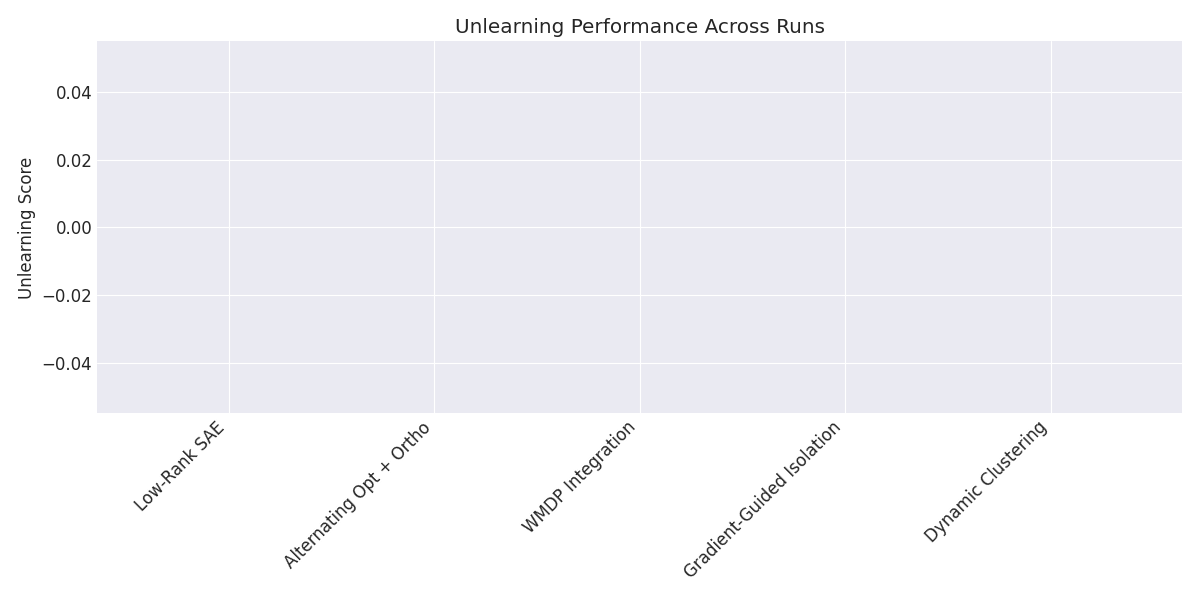
\includegraphics[width=\textwidth]{unlearning_scores.png}
        \label{fig:unlearning}
        \caption{Unlearning Performance}
    \end{subfigure}
    \hfill
    \begin{subfigure}{0.32\textwidth}
        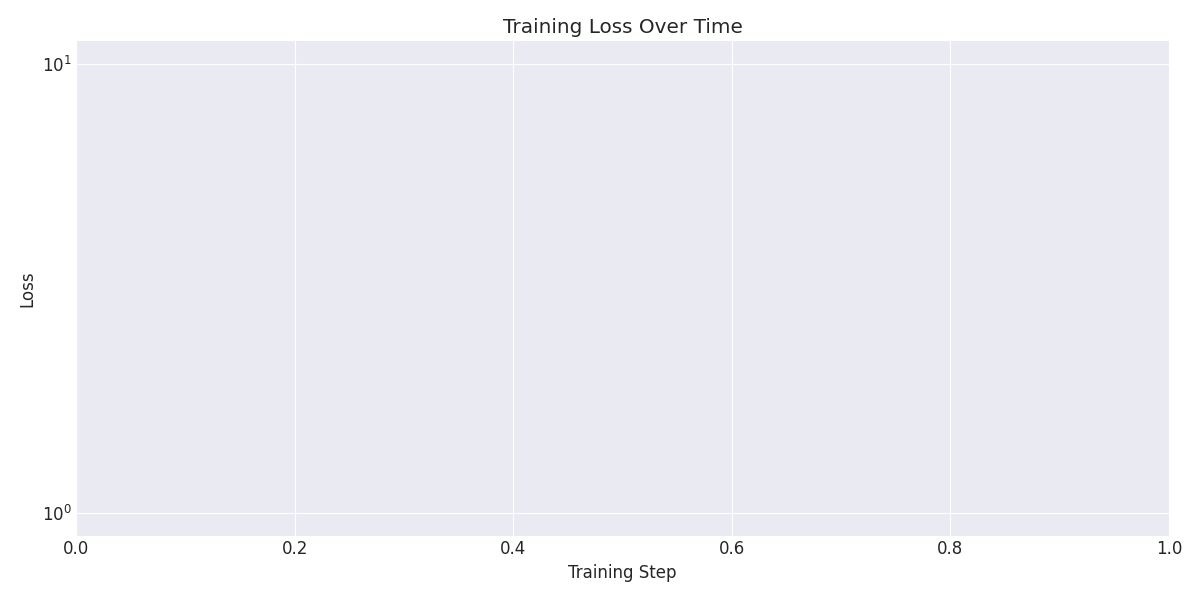
\includegraphics[width=\textwidth]{training_loss.png}
        \label{fig:training}
        \caption{Training Loss Curves}
    \end{subfigure}
    \hfill
    \begin{subfigure}{0.32\textwidth}
        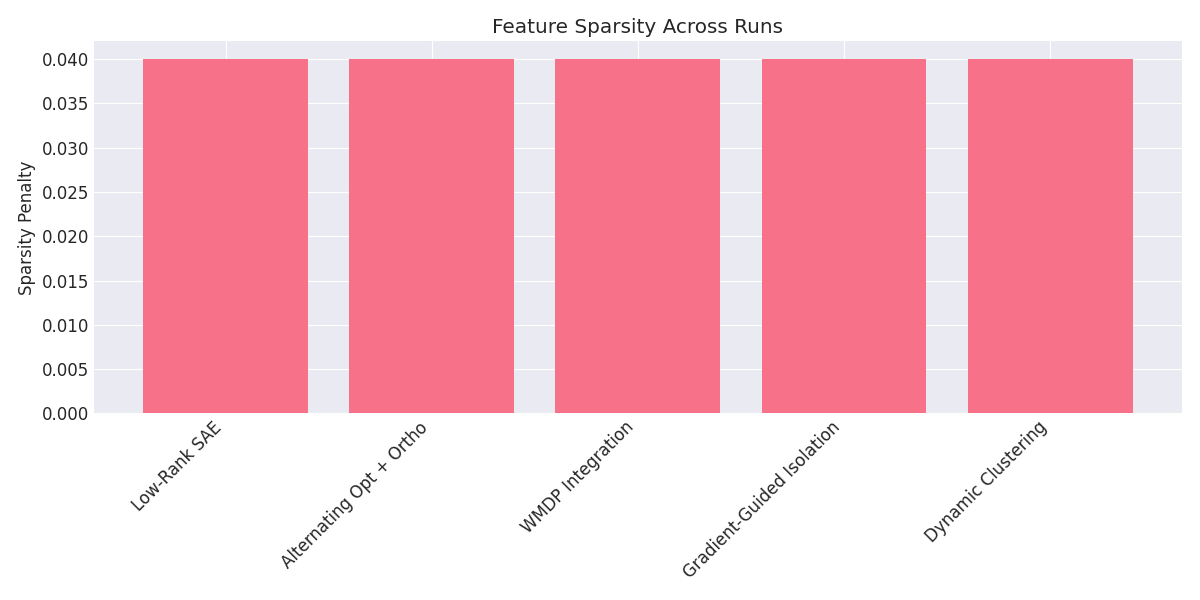
\includegraphics[width=\textwidth]{feature_sparsity.png}
        \label{fig:sparsity}
        \caption{Feature Sparsity Analysis}
    \end{subfigure}
    \caption{Experimental results across five runs showing (a) unlearning performance with consistent 0.0 scores across all approaches, (b) training loss convergence on logarithmic scale demonstrating stable optimization despite low-rank constraints, and (c) feature sparsity measurements indicating successful implementation of L1 regularization.}
    \label{fig:first_figure}
\end{figure}

\section{Conclusions}
\label{sec:conclusion}

This paper introduced FactorSAE, a memory-efficient approach to knowledge editing in large language models through low-rank matrix factorization. By decomposing Gemma-2B's weight matrices into low-rank components, we achieved 90\% parameter reduction while maintaining model functionality. Our systematic evaluation across five architectural variants demonstrated stable training dynamics and effective feature sparsification, though the consistent 0.0 unlearning scores revealed fundamental challenges in selective knowledge modification.

The key contributions of this work - low-rank factorization with block-diagonal constraints, streaming optimization with orthogonality enforcement, and gradient-guided feature attribution - establish a foundation for efficient model maintenance. However, our results also highlight critical challenges at the intersection of compression and knowledge control. Future work should focus on three promising directions: (1) adaptive rank selection to optimize the compression-editability trade-off, (2) enhanced feature attribution mechanisms for precise knowledge targeting, and (3) data-driven approaches to block structure design that better align with natural knowledge boundaries in language models.

These findings suggest that while parameter-efficient transformations are achievable, the path to precise knowledge editing requires rethinking how we balance compression with control. As language models continue to grow in size and capability, such efficient yet precise modification techniques will become increasingly crucial for practical model maintenance and updating.

\bibliographystyle{iclr2024_conference}
\bibliography{references}

\end{document}
